\documentclass[9pt]{extarticle}
\usepackage[margin=0.3in]{geometry}
\usepackage{multicol}
\usepackage{amsmath}
\usepackage{tikz}
\usepackage{xcolor}
\usepackage{hyperref}
\usepackage{graphicx}
\setlength{\parindent}{0pt}
\pagestyle{empty}
\definecolor{sectioncolor}{HTML}{003366}
\definecolor{subsectioncolor}{HTML}{006699}
\definecolor{highlight}{HTML}{990000}
\begin{document}
\small
\begin{multicols*}{3}
% --------------------------------------------------------------------
% Introduction to Networking
% --------------------------------------------------------------------
\begin{center}
    {\Large\textbf{Introduction to Networking}}\\
    Ramesh Govindan\\
    August 26, 2024
\end{center}

% --------------------------------------------------------------------
% Acknowledgements
% --------------------------------------------------------------------
{\color{sectioncolor}\section*{\centering Acknowledgements}}
All materials for this course adapted from courses developed by Morley Mao, Mosharaf Chowdhury, Aditya Akella, Sugih Jamin, Philip Levis, Sylvia Ratnasamy, Peter Steenkiste, and many other colleagues.

Many figures and slides borrowed from Jim Kurose and Keith Ross's textbook and slides.

\textbf{Recommended Textbook}

% --------------------------------------------------------------------
% A Data Network
% --------------------------------------------------------------------
{\color{sectioncolor}\section*{\centering A Data Network}}
Consists of:
\begin{itemize}
    \item \textbf{Links} that interconnect
    \item \textbf{Hosts} and \textbf{Routers} in order to
    \begin{itemize}
        \item Move data between hosts via routers
        \item Hosts also called \textbf{End Systems}
        \item Routers sometimes called \textbf{Switches}
    \end{itemize}
\end{itemize}

% Diagram Placeholder
\begin{center}
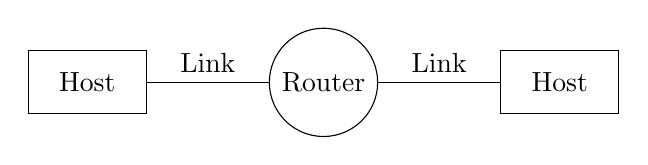
\begin{tikzpicture}[node distance=2cm, auto]
    \node[draw, rectangle, minimum width=1.5cm, minimum height=0.8cm] (host1) {Host};
    \node[draw, circle, right of=host1, node distance=3cm] (router) {Router};
    \node[draw, rectangle, minimum width=1.5cm, minimum height=0.8cm, right of=router, node distance=3cm] (host2) {Host};
    \draw[-] (host1) -- node[above]{Link} (router);
    \draw[-] (router) -- node[above]{Link} (host2);
\end{tikzpicture}
\end{center}

\textbf{The Internet}
\begin{itemize}
    \item A large, global, data network
    \item Focus of this class
\end{itemize}

% --------------------------------------------------------------------
% A Macroscopic View
% --------------------------------------------------------------------
{\color{sectioncolor}\section*{\centering A Macroscopic View}}
How hosts connect to the network:

\textbf{Hosts}
\begin{itemize}
    \item Laptops
    \item Smartphones
    \item Other smart devices
\end{itemize}

\textbf{Links}
\begin{itemize}
    \item Wired
    \item Wireless
\end{itemize}

% Diagram Placeholder
\begin{center}
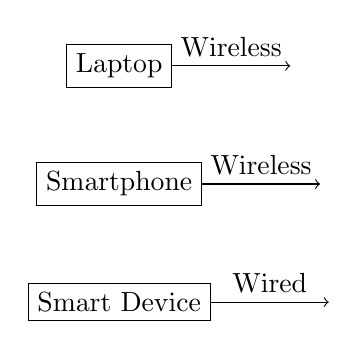
\begin{tikzpicture}[node distance=1.5cm, auto]
    \node[draw, rectangle] (laptop) {Laptop};
    \node[draw, rectangle, below of=laptop] (smartphone) {Smartphone};
    \node[draw, rectangle, below of=smartphone] (device) {Smart Device};
    \draw[->] (laptop.east) -- ++(1.5cm,0) node[midway, above]{Wireless};
    \draw[->] (smartphone.east) -- ++(1.5cm,0) node[midway, above]{Wireless};
    \draw[->] (device.east) -- ++(1.5cm,0) node[midway, above]{Wired};
\end{tikzpicture}
\end{center}

% --------------------------------------------------------------------
% Networks and Routers
% --------------------------------------------------------------------
{\color{sectioncolor}\section*{\centering Networks and Routers}}
\textbf{Routers}
\begin{itemize}
    \item Wireless access points
    \item Cell towers
    \item Wired switches
\end{itemize}

\textbf{Networks}
\begin{itemize}
    \item Local ISPs
    \item Campus networks
    \item National ISPs
\end{itemize}

% --------------------------------------------------------------------
% A Shared Network
% --------------------------------------------------------------------
{\color{sectioncolor}\section*{\centering A Shared Network}}
\textbf{Sharing!}
\begin{itemize}
    \item Apps and hosts share routers and links
    \item Red and blue traffic go over the same link
\end{itemize}

% Diagram Placeholder
\begin{center}
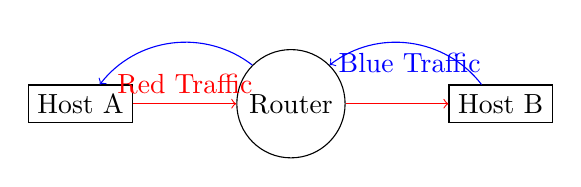
\begin{tikzpicture}
    \node[draw, circle] (router) {Router};
    \node[draw, rectangle, left=2cm] (host1) {Host A};
    \node[draw, rectangle, right=2cm] (host2) {Host B};
    \draw[->, red] (host1) -- node[above]{Red Traffic} (router);
    \draw[->, red] (router) -- (host2);
    \draw[->, blue, bend right=45] (host2) to node[below]{Blue Traffic} (router);
    \draw[->, blue, bend right=45] (router) to (host1);
\end{tikzpicture}
\end{center}

% --------------------------------------------------------------------
% Two Ways to Share Switched Networks
% --------------------------------------------------------------------
{\color{sectioncolor}\section*{\centering Two Ways to Share Switched Networks}}
\begin{itemize}
    \item \textbf{Circuit Switching}
    \item \textbf{Packet Switching}
\end{itemize}

% --------------------------------------------------------------------
% Circuit Switching
% --------------------------------------------------------------------
{\color{sectioncolor}\section*{\centering Circuit Switching}}
\textbf{What is it?}
\begin{itemize}
    \item Circuit: a connection between sender and receiver with dedicated resources
    \item Analogy: multiple lanes between each pair of routers; circuit uses one of these lanes at each hop
\end{itemize}

\textbf{How is it implemented?}
\begin{itemize}
    \item \textbf{Frequency-Division Multiplexing (FDM)}
    \begin{itemize}
        \item Optical cables have different frequencies
        \item Each circuit sent on a different frequency
    \end{itemize}
    \item \textbf{Time-Division Multiplexing (TDM)}
    \begin{itemize}
        \item Data from different connections sent in different time slots
    \end{itemize}
\end{itemize}

% --------------------------------------------------------------------
% Packet Switching
% --------------------------------------------------------------------
{\color{sectioncolor}\section*{\centering Packet Switching}}
\textbf{What is a packet?}
\begin{itemize}
    \item A unit of data transmitted on network
    \item Have a maximum size (\( L \) bits)
    \item Large transfers divided into multiple packets
\end{itemize}

\textbf{What do routers do with packets?}
\begin{itemize}
    \item \textbf{Store and Forward}
    \begin{itemize}
        \item Router waits to receive full packet
        \item Stores it locally
        \item Forwards it towards destination
    \end{itemize}
\end{itemize}

\textbf{Queueing at routers}
\begin{itemize}
    \item \textbf{Queue}: a sequence of packets stored in a router waiting to be transmitted
    \item Queues form when packets arrive faster than can be sent out
    \item If queue is large, router may drop packets
\end{itemize}

% --------------------------------------------------------------------
% Which Is Better? Pros and Cons
% --------------------------------------------------------------------
{\color{sectioncolor}\section*{\centering Which Is Better? Pros and Cons}}
\textbf{Circuit Switching}
\begin{itemize}
    \item \textbf{Pros}
    \begin{itemize}
        \item Predictable performance
        \item Simple/fast switching (once circuit established)
    \end{itemize}
    \item \textbf{Cons}
    \begin{itemize}
        \item Complexity and delay of circuit setup/teardown
        \item If switch fails, its circuit(s) fail
    \end{itemize}
\end{itemize}

\textbf{Packet Switching}
\begin{itemize}
    \item \textbf{Pros}
    \begin{itemize}
        \item No circuit setup, faster transfers
        \item Easier failure handling, re-route on different path
    \end{itemize}
    \item \textbf{Cons}
    \begin{itemize}
        \item Packets can be dropped, impacting performance
        \item Queueing can add delays
    \end{itemize}
\end{itemize}

% --------------------------------------------------------------------
% Statistical Multiplexing
% --------------------------------------------------------------------
{\color{sectioncolor}\section*{\centering Statistical Multiplexing}}
\textbf{Why the Internet uses packet switching}
\begin{itemize}
    \item Computer communication is bursty
    \item Applications/services have on/off behavior
    \item Packet-switched networks can more efficiently support bursty traffic due to statistical multiplexing
\end{itemize}

\textbf{An Example}
\begin{itemize}
    \item Circuit switching can only support 10 users; must build network for worst case
    \item Packet switching can support 35 users because probability that all users are active at the same time is low
\end{itemize}

% --------------------------------------------------------------------
% Measures of Network Performance
% --------------------------------------------------------------------
{\color{sectioncolor}\section*{\centering Measures of Network Performance}}
\begin{enumerate}
    \item End-to-end delay
    \item Packet loss rate
    \item Throughput
\end{enumerate}

% --------------------------------------------------------------------
% End-to-end Delay
% --------------------------------------------------------------------
{\color{sectioncolor}\section*{\centering End-to-end Delay}}
Let:
\begin{itemize}
    \item \( t_{\text{sent}} \) be time sent
    \item \( t_{\text{recv}} \) be time received
\end{itemize}
End-to-end delay:
\[
d_{\text{end-to-end}} = t_{\text{recv}} - t_{\text{sent}}
\]

\textbf{Components of End-to-end Delay}
\begin{itemize}
    \item \textbf{Transmission Delay} (\( d_{\text{trans}} \))
    \item \textbf{Propagation Delay} (\( d_{\text{prop}} \))
    \item \textbf{Queueing Delay} (\( d_{\text{queue}} \))
    \item \textbf{Processing Delay} (\( d_{\text{proc}} \))
\end{itemize}
Total delay at a router:
\[
d_{\text{router}} = d_{\text{queue}} + d_{\text{proc}} + d_{\text{trans}} + d_{\text{prop}}
\]

% --------------------------------------------------------------------
% Packet Loss Rate
% --------------------------------------------------------------------
{\color{sectioncolor}\section*{\centering Packet Loss Rate}}
Let:
\begin{itemize}
    \item \( N \) be number of packets sent
    \item \( l \) be number of packets lost
    \item \( p \) be packet loss rate
\end{itemize}
Packet loss rate:
\[
p = \frac{l}{N}
\]

\textbf{Recovering from packet loss}
\begin{itemize}
    \item Hosts/applications detect when a packet is lost
    \item Retransmit lost packets to recover from loss
\end{itemize}

% --------------------------------------------------------------------
% Throughput
% --------------------------------------------------------------------
{\color{sectioncolor}\section*{\centering Throughput}}
\textbf{Definitions}
\begin{itemize}
    \item If \( B \) bits are transferred from sender to receiver in time \( t \), then:
    \[
    \text{Throughput} = \frac{B}{t}
    \]
    \item \textbf{Instantaneous Throughput}: when \( t \) is small
    \item \textbf{Average Throughput}: over the duration of a connection
\end{itemize}

% Continue from where we left off
% --------------------------------------------------------------------
% Pipe Model of a Link
% --------------------------------------------------------------------
{\color{sectioncolor}\section*{\centering Pipe Model of a Link}}
\textbf{What is a model?}
\begin{itemize}
    \item A mathematical or mental construct that helps understand a physical process
\end{itemize}
\textbf{Pipe Model}
\begin{itemize}
    \item A link is modeled as a pipe (though it doesn't carry water!)
    \item Helps us understand link behavior
\end{itemize}
Will use this model later in the course.

% --------------------------------------------------------------------
% Queueing
% --------------------------------------------------------------------
{\color{sectioncolor}\section*{\centering Queueing}}
\textbf{Why do queues form at routers?}
\begin{itemize}
    \item If packets arrive faster than the router can process, they are placed into a queue
    \item \textbf{Queueing delay}:
    \begin{itemize}
        \item \( t_{p,e} \): time when packet \( p \) enters queue
        \item \( t_{p,l} \): time when it leaves queue
        \item \( d_{\text{queue}} = t_{p,l} - t_{p,e} \)
    \end{itemize}
    \item Transient overload when packets are queued
\end{itemize}

\textbf{When do queues never form?}
\begin{itemize}
    \item If router can process and send packets faster than they arrive, no queues form
\end{itemize}

\textbf{When can a router drop packets?}
\begin{itemize}
    \item If router runs out of memory (buffer), it may drop a packet
\end{itemize}

% --------------------------------------------------------------------
% Queueing Delay
% --------------------------------------------------------------------
{\color{sectioncolor}\section*{\centering Queueing Delay}}
Per-packet queueing delay:
\[
d_{\text{queue}} = t_{p,l} - t_{p,e}
\]
Characterized by statistical measures:
\begin{itemize}
    \item Average queueing delay
    \item Variance of queueing delay
    \item Probability delay exceeds a threshold value
\end{itemize}

\textbf{Queueing Theory}
\begin{itemize}
    \item Complex mathematical discipline studying queue behavior under different conditions
    \item \textbf{Little's Law}:
    \[
    L = \lambda \times W
    \]
    \begin{itemize}
        \item \( L \): Average length of queue
        \item \( \lambda \): Average arrival rate
        \item \( W \): Average wait time
    \end{itemize}
    \item Independent of arrival pattern and service times
\end{itemize}

% --------------------------------------------------------------------
% Processing Delay
% --------------------------------------------------------------------
{\color{sectioncolor}\section*{\centering Processing Delay}}
\begin{itemize}
    \item Router processing involves reading and possibly modifying the packet
    \item \( d_{\text{proc}} \) is usually negligible
\end{itemize}

% --------------------------------------------------------------------
% End-to-End Delay
% --------------------------------------------------------------------
{\color{sectioncolor}\section*{\centering End-to-End Delay}}
Delay at router:
\[
d_{\text{router}} = d_{\text{queue}} + d_{\text{proc}} + d_{\text{trans}} + d_{\text{prop}}
\]
End-to-end delay:
\[
d_{\text{end-to-end}} = \sum_{\text{routers}} d_{\text{router}}
\]
Why do delays add up?
\begin{itemize}
    \item Store-and-forward routers wait to receive the full packet before processing
\end{itemize}

% --------------------------------------------------------------------
% Summary
% --------------------------------------------------------------------
{\color{sectioncolor}\section*{\centering Summary}}
\begin{itemize}
    \item \textbf{Elements of Network}: Links, hosts, routers
    \item \textbf{Internet}: Network of networks
    \item \textbf{Sharing}: Circuit vs. packet switching
    \item \textbf{Packet Switching}: Multiplexing, packet loss, queueing
    \item \textbf{Measures}: Loss rate, delay, throughput
\end{itemize}

% --------------------------------------------------------------------
% Additional Reading
% --------------------------------------------------------------------
{\color{sectioncolor}\section*{\centering Additional Reading}}
\begin{itemize}
    \item Sections 1.1, 1.3, 1.4 from the recommended textbook
\end{itemize}

% --------------------------------------------------------------------
% Layering and Protocols
% --------------------------------------------------------------------
{\color{sectioncolor}\section*{\centering Layering and Protocols}}
Ramesh Govindan\\
September 3, 2024

% Continue with the next sections following the same structure...

% --------------------------------------------------------------------
% The Web
% --------------------------------------------------------------------
{\color{sectioncolor}\section*{\centering The Web}}
Ramesh Govindan\\
September 4, 2024

\textbf{Widely-used Networked Applications}
\begin{itemize}
    \item \textbf{Communication}: E-mail, Text messaging, Social networking
    \item \textbf{Entertainment}: Gaming, Video streaming (e.g., YouTube)
    \item \textbf{Information}: Web, Internet Search
    \item \textbf{Telepresence}: Voice over IP, Video conferencing (e.g., Zoom)
\end{itemize}
Will learn later how many of these work.

% --------------------------------------------------------------------
% What is the Web?
% --------------------------------------------------------------------
{\color{sectioncolor}\section*{\centering What is the Web?}}
\textbf{The Logical View}
\begin{itemize}
    \item Database of hypertext documents
    \item Origins in the 90s by Tim Berners-Lee at CERN to facilitate scientific collaboration
\end{itemize}

\textbf{Hypertext and Hyperlinks}
\begin{itemize}
    \item \textbf{Hypertext}: Text containing hyperlinks
    \item \textbf{Hyperlink}: Reference to another document or object
\end{itemize}

\textbf{Hypertext Markup Language (HTML)}
\begin{itemize}
    \item Language for marking up text
    \item Markups for formatting and hyperlinks
\end{itemize}

% --------------------------------------------------------------------
% How it Works
% --------------------------------------------------------------------
{\color{sectioncolor}\section*{\centering How it Works}}
\textbf{User} types URL into browser.

\textbf{Browser}
\begin{itemize}
    \item Sends request to server over the Internet
\end{itemize}

\textbf{Server}
\begin{itemize}
    \item Responds with page contents
\end{itemize}

% Continue integrating the rest of the provided text, maintaining the same structure and formatting.

% Remember to include any mathematical expressions, diagrams, or placeholders as necessary.

% --------------------------------------------------------------------
% End of Document
% --------------------------------------------------------------------

\end{multicols*}
\end{document}